\documentclass[12pt]{article}
\usepackage{algos-tasks}
\usepackage{listings}
\usepackage[table]{xcolor}
\usepackage{array}
\usepackage{xcolor} % pretty colours
\usepackage{varwidth}
\title{2.3 Art Gallery}
\author{Andre Monteiro}
\date{Term 3, 2025}

\begin{document}
\maketitle
\newpage
\subsection*{Problem Summary}
Given a sorted array
\[
P = [p_1, p_2,\ldots, p_n]
\]

of $n$ real numbers representing the positions of paintings along a hallway, determine the minimum number of guards required to protect all paintings. Each guard can protect any painting located within a distance of 1 unit to their left or right (i.e., a total coverage of 2 units). The goal is to compute the optimal placement of guards such that all paintings are protected while minimizing the number of guards used.
\begin{center}
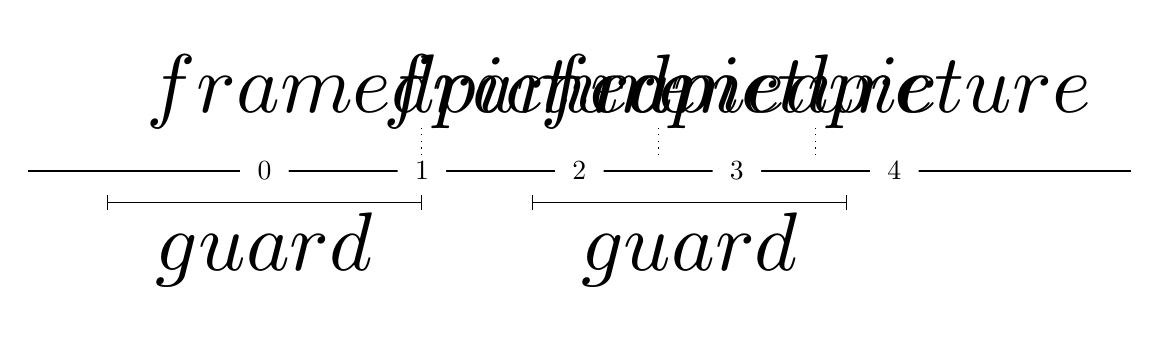
\begin{tikzpicture}
	\draw (-3,0) -- (11,0);
	\begin{scope}[every node/.style={circle, fill=white}]
		\node at (0,0) {$0$};
		\node at (2,0) {$1$};
		\node at (4,0) {$2$};
		\node at (6,0) {$3$};
		\node at (8,0) {$4$};
	\end{scope}
	\begin{scope}[every node/.style={scale=3}]
		\foreach \p in {2,5,7} {
			\node at (\p,1) {$\texttwemoji{framed picture}$};
			\draw[dotted] (\p,0.2) -- (\p,0.6);
		}
		\foreach \g in {0,5.4} {
			\node at (\g,-1) {$\texttwemoji{guard}$};
			\draw[|-|] (\g-2,-0.4) -- (\g+2,-0.4);
		}
	\end{scope}
\end{tikzpicture}
\end{center}
\newpage
\subsection*{Question a)}
The art gallery also presents Larry with one potential strategy to protect the paintings:
\begin{center}
\textit{``Place a guard one unit to the left of the leftmost unprotected painting, and repeat.''}
\end{center}

To demonstrate that the given algorithm does not always yield an optimal solution, consider the following example:

Let \( N = 3 \), representing 3 paintings, with positions given by the array:
\[
P = [1, 2, 3]
\]

According to the algorithm, we place the first guard \textit{one unit to the left} of the leftmost unguarded painting. Since the first painting is located at position 1, the guard is placed at position 0:

\begin{center}
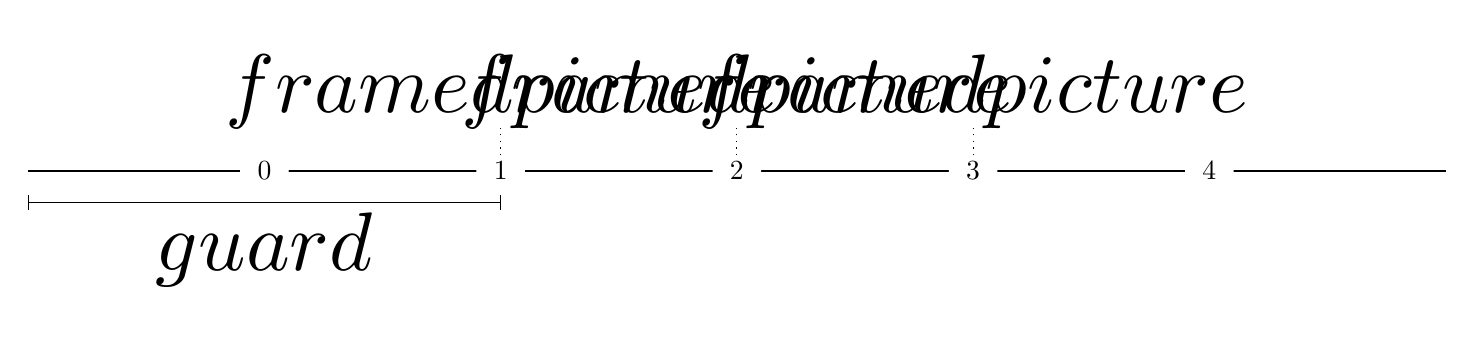
\begin{tikzpicture}
	\draw (-5,0) -- (13,0);
	\begin{scope}[every node/.style={circle, fill=white}]
		\node at (-2,0) {$0$};
		\node at (1,0) {$1$};
		\node at (4,0) {$2$};
		\node at (7,0) {$3$};
		\node at (10,0) {$4$};
	\end{scope}
	\begin{scope}[every node/.style={scale=3}]
		\foreach \p in {1,4,7} {
			\node at (\p,1) {$\texttwemoji{framed picture}$};
			\draw[dotted] (\p,0.2) -- (\p,0.6);
		}
		\foreach \g in {-2} {
			\node at (\g,-1) {$\texttwemoji{guard}$};
			\draw[|-|] (\g-3,-0.4) -- (\g+3,-0.4);
		}
	\end{scope}
\end{tikzpicture}
\end{center}

After placing the first guard, the algorithm proceeds by discarding the paintings already covered and repeating the same step for the next leftmost unguarded painting. The process continues as follows:

\begin{center}
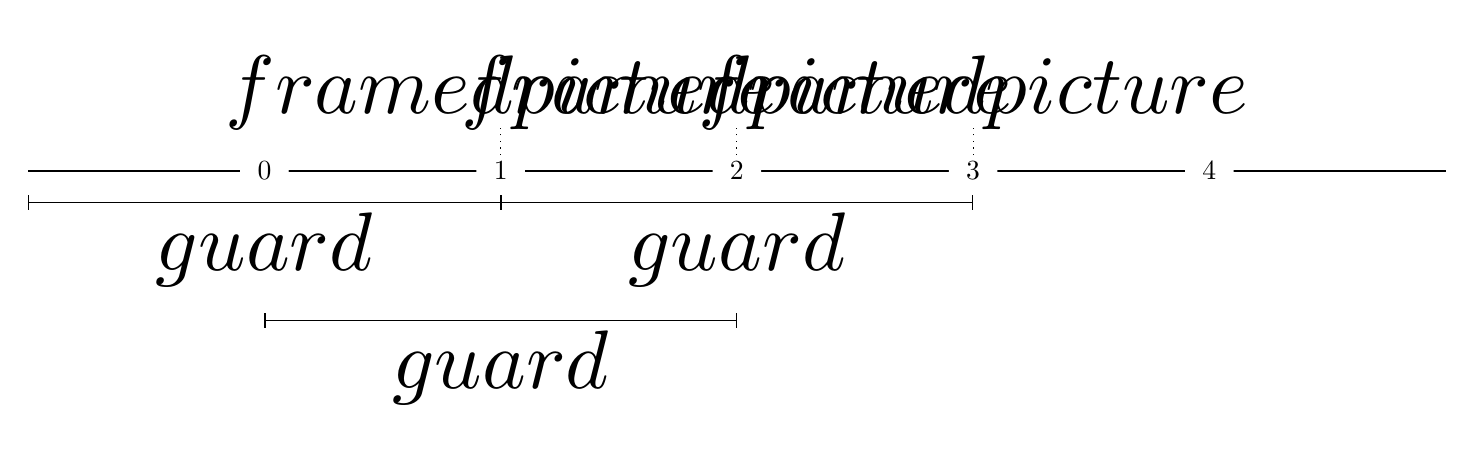
\begin{tikzpicture}
	\draw (-5,0) -- (13,0);
	\begin{scope}[every node/.style={circle, fill=white}]
		\node at (-2,0) {$0$};
		\node at (1,0) {$1$};
		\node at (4,0) {$2$};
		\node at (7,0) {$3$};
		\node at (10,0) {$4$};
	\end{scope}
	\begin{scope}[every node/.style={scale=3}]
		\foreach \p in {1,4,7} {
			\node at (\p,1) {$\texttwemoji{framed picture}$};
			\draw[dotted] (\p,0.2) -- (\p,0.6);
		}
		\foreach \g in {-2,4} {
			\node at (\g,-1) {$\texttwemoji{guard}$};
			\draw[|-|] (\g-3,-0.4) -- (\g+3,-0.4);
		}
        \foreach \g in {1} {
			\node at (\g,-2.5) {$\texttwemoji{guard}$};
			\draw[|-|] (\g-3,-1.9) -- (\g+3,-1.9);
		}
	\end{scope}
\end{tikzpicture}
\end{center}
As a result, the algorithm places \textbf{three guards}, one for each painting, even though it is possible to protect all three paintings using only one guard, for example by placing a guard at position 2. This demonstrates that the algorithm is not optimal in all cases.

\begin{center}
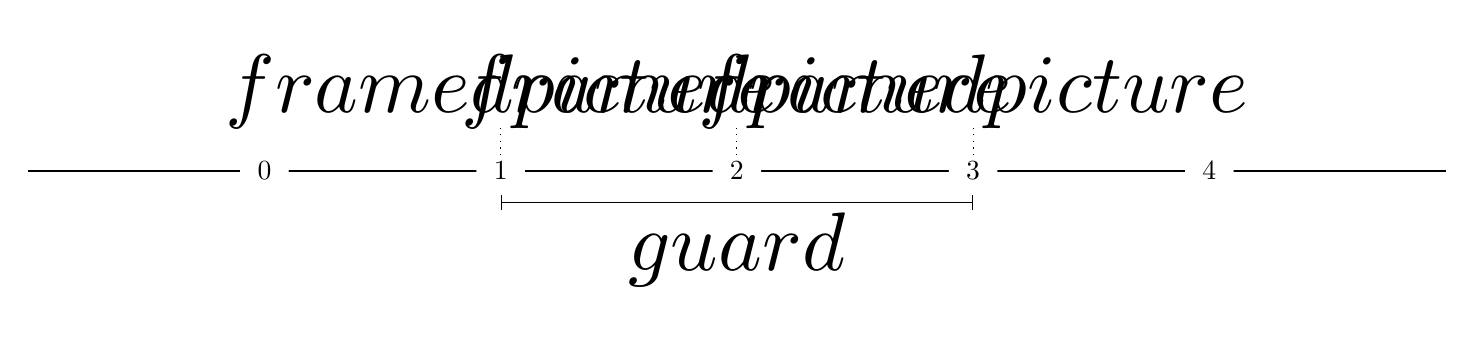
\begin{tikzpicture}
	\draw (-5,0) -- (13,0);
	\begin{scope}[every node/.style={circle, fill=white}]
		\node at (-2,0) {$0$};
		\node at (1,0) {$1$};
		\node at (4,0) {$2$};
		\node at (7,0) {$3$};
		\node at (10,0) {$4$};
	\end{scope}
	\begin{scope}[every node/.style={scale=3}]
		\foreach \p in {1,4,7} {
			\node at (\p,1) {$\texttwemoji{framed picture}$};
			\draw[dotted] (\p,0.2) -- (\p,0.6);
		}
		\foreach \g in {4} {
			\node at (\g,-1) {$\texttwemoji{guard}$};
			\draw[|-|] (\g-3,-0.4) -- (\g+3,-0.4);
		}
        
	\end{scope}
\end{tikzpicture}
\end{center}
\newpage
\subsection*{Question b)}
To better optimize the provided implementation, the gallery shoudl instead position the guard one unit to the right, as follows: 

Let \( N = 3 \), representing 3 paintings, with positions given by the array:
\[
P = [1, 2, 3]
\]
After placing the first guard, the algorithm proceeds by removing the paintings already covered and repeating the same process for the next leftmost unguarded painting. This continues until all paintings are protected.

\begin{center}
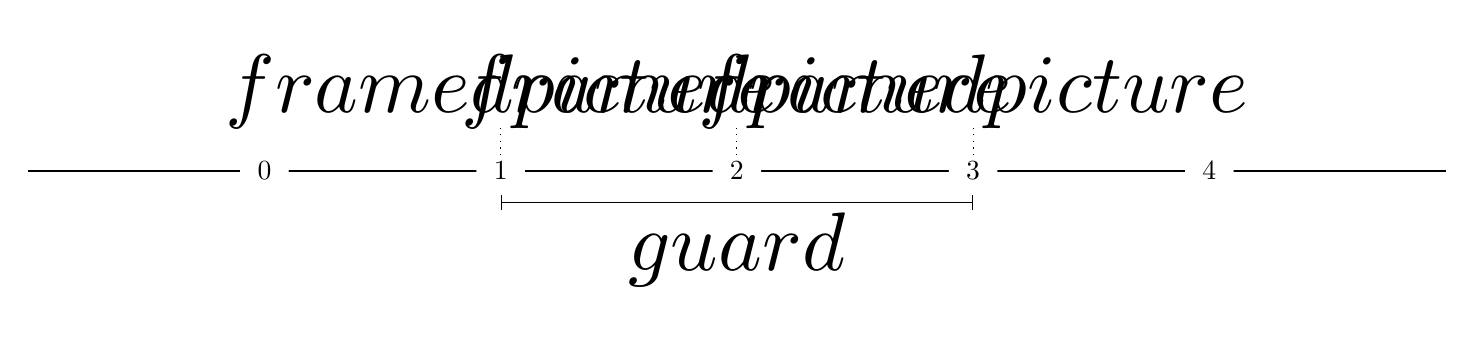
\begin{tikzpicture}
	\draw (-5,0) -- (13,0);
	\begin{scope}[every node/.style={circle, fill=white}]
		\node at (-2,0) {$0$};
		\node at (1,0) {$1$};
		\node at (4,0) {$2$};
		\node at (7,0) {$3$};
		\node at (10,0) {$4$};
	\end{scope}
	\begin{scope}[every node/.style={scale=3}]
		\foreach \p in {1,4,7} {
			\node at (\p,1) {$\texttwemoji{framed picture}$};
			\draw[dotted] (\p,0.2) -- (\p,0.6);
		}
		\foreach \g in {4} {
			\node at (\g,-1) {$\texttwemoji{guard}$};
			\draw[|-|] (\g-3,-0.4) -- (\g+3,-0.4);
		}
	\end{scope}
\end{tikzpicture}
\end{center}

As such, the algorithm places \textbf{one guard}, which is indeed the optimal solution.

\subsection*{Correctness Argument (Through induction)}

We aim to prove that the greedy algorithm correctly places the minimum number of guards required to protect all paintings, given that each guard covers a range of 2 units (from \( x - 1 \) to \( x + 1 \)).

\paragraph{Claim:}  
The greedy algorithm always produces an optimal (i.e., minimal) number of guards to cover all paintings in the array \( P = [p_1, p_2, \dots, p_n] \), where \( p_i \) represents the position of the \( i^{\text{th}} \) painting.

\paragraph{Base Case (1 painting):}  
If there is only one painting, the algorithm places a guard at position \( p_1 + 1 \), which covers the interval \( [p_1, p_1 + 2] \) and thus protects the painting. Since any valid solution must use at least one guard to cover one painting, the algorithm is clearly optimal in this case.

\paragraph{Inductive Hypothesis:}  
Assume that for any sorted list of \( k \) paintings (where \( 1 \leq k < n \)), the greedy algorithm places the minimum number of guards necessary to cover all \( k \) paintings.

\paragraph{Inductive Step:}  
We now prove that the algorithm also places the minimum number of guards for \( k + 1 \) paintings.

Let \( p_i \) be the leftmost unprotected painting.  
The algorithm places a guard at position \( p_i + 1 \), which protects paintings in the interval \( [p_i, p_i + 2] \). It then proceeds to the next unprotected painting and repeats the process.

Consider the last painting in the sequence, \( p_{k+1} \), and examine the two possibilities:

\begin{itemize}
    \item \textbf{Case 1:} \( p_{k+1} \) is already covered by a guard placed earlier. \\
    In this case, the inductive hypothesis guarantees that all previous paintings (including \( p_{k+1} \)) have already been covered using the minimum number of guards. No additional guard is needed, so the algorithm remains optimal.

    \item \textbf{Case 2:} \( p_{k+1} \) is not yet covered. \\
    Then the algorithm places a guard at \( p_{k+1} + 1 \), covering the interval \( [p_{k+1}, p_{k+1} + 2] \). 

    Suppose there exists an alternative solution that uses fewer guards to cover all \( k+1 \) paintings. Since \( p_{k+1} \) is not covered by previous guards, any valid solution must place an additional guard to protect it. Placing this guard at any position other than \( p_{k+1} + 1 \) either (1) fails to cover \( p_{k+1} \), or (2) covers fewer paintings than the greedy placement. Hence, the greedy choice is at least as good as any alternative.
\end{itemize}

In either case, the greedy algorithm uses no more guards than any alternative, maintaining optimality.

\paragraph{Conclusion:}  
By the principle of mathematical induction, the greedy algorithm places the minimum number of guards needed to protect any number of paintings. Therefore, the algorithm is correct and optimal.

\newpage
\subsection*{Time Complexity}

The algorithm performs a single pass over the sorted array of painting positions:

\begin{itemize}
    \item At each step, it selects the leftmost unprotected painting.
    \item It places a guard to cover as many paintings as possible within the 2-unit range.
    \item It skips over all paintings that are now protected.
\end{itemize}

Each painting is checked at most once, and each guard placement is a constant-time operation. There are no nested loops or recursive steps.

\paragraph{Therefore, the total time complexity is:}
\[
\boxed{O(n)}
\]

where \( n \) is the number of paintings. Even in the worst-case scenario, where each painting is more than 2 units apart and requires its own guard, the algorithm still only makes one linear pass.

\end{document}